\documentclass[10pt,twocolumn,letterpaper]{article}

\usepackage{cvpr}
\usepackage{times}
\usepackage{epsfig}
\usepackage{graphicx}
\usepackage{amsmath}
\usepackage{amssymb}

\usepackage{booktabs} % For midrules

\usepackage[table]{xcolor}

\renewcommand*\thetable{\Roman{table}}

\usepackage{titling}
\setlength{\droptitle}{-1em}   % This is your set screw

% Include other packages here, before hyperref.

% If you comment hyperref and then uncomment it, you should delete
% egpaper.aux before re-running latex.  (Or just hit 'q' on the first latex
% run, let it finish, and you should be clear).
\usepackage[breaklinks=true,bookmarks=false,colorlinks=true,linkcolor=blue,allcolors=blue]{hyperref}

\cvprfinalcopy % *** Uncomment this line for the final submission

\def\cvprPaperID{****} % *** Enter the CVPR Paper ID here
\def\httilde{\mbox{\tt\raisebox{-.5ex}{\symbol{126}}}}

% Pages are numbered in submission mode, and unnumbered in camera-ready
%\ifcvprfinal\pagestyle{empty}\fi
%\setcounter{page}{4321}
\begin{document}

%%%%%%%%% TITLE
\title{Financial Time Series Prediction with Deep Learning}

\author{Alex Carrillo Alza\\
{\tt\small alex.carrillo.alza@estudiantat.upc.edu}
% For a paper whose authors are all at the same institution,
% omit the following lines up until the closing ``}''.
% Additional authors and addresses can be added with ``\and'',
% just like the second author.
% To save space, use either the email address or home page, not both
\and
Advisor: Prof. J. A. Rodríguez\\
{\tt\small jose.fonollosa@upc.edu}
\and
January 2021, \textit{Universitat Politècnica de Catalunya}\\
}

\date{\vspace{-5ex}}

\maketitle
%\thispagestyle{empty}

%%%%%%%%% ABSTRACT
\begin{abstract}
	This work presents a study on the application of state-of-art language modeling deep learning architectures to the analysis of financial time series. First, after a short introduction to the topic, the article reviews the main deep computing-based trading methods in the literature: Recurrent Neural Networks (RNNs; primarily the Long Short-Term Memory, LSTM architecture), Convolutional Neural Networks (CNNs) and related work. Second, the paper describes the implementation of an LSTM network by gently illustrating the variety of concerns it entails, and gives examples of how this model could be able to provide profitable predictions of cryptocurrencies' price trends such as Bitcoin.
\end{abstract}

%%%%%%%%% BODY TEXT
\section{Introduction and Motivation}

In the last decade, the first cryptocurrency ever created and the most widely used alternative currency, Bitcoin \cite{bitcoin}, has experienced an unprecedented growth and captivated the interest of new investors on the financial market. At the time this report was written, Bitcoin’s worth price reached close to 30,000 USD. This new market niche can be directly compared to the stock, forex and derivatives market (futures, swaps, options) and essentially the same tools and analysis can be used to forecast price trends for profit-maximization.

The price of a share or a commodity is explained by the law of supply and demand between investors and holders and, at the same time, the demand of investors responds to the perceptions of the evolution of a company or the worth of a good in the future. Thus, 1- investors seek to earn a return on their shares; 2- the outcome of an asset obtained in the past has already impacted on the past demand and it is reflected in the current price; 3- future forecasts will determine the expected profitability of investors and the intensity of demand.

It is worth mentioning that there originally exist two main approaches in stock (and also cryptocurrency) price analysis. On the one hand, fundamental analysis aims to obtain the intrinsic value of an asset and states that its price will tend to its objective price. In order to achieve the above, in this type of medium-long term analysis \textit{fundamentalists} focus on the economic situation, the performance of a company or the usability, adoption and government regulations, \ie looking for the \textit{cause} of the price. On the other hand, technical analysis aims to obtain a predictable behaviour of an asset and claims that markets repeat behaviors over time. In this type of short-medium term analysis \textit{chartists} focus on charts’ shapes, technical indicators and oscillators, \ie studying the \textit{consequences} of variations in the price.

It must be taken into account there is a steady discussion about the futile use of technical trading strategies regarding the predictability of the stock markets, cryptocurrencies or other assets. The above is essentially justified by the intrinsic difficulty of market behaviour: stochastic, dynamic, volatile and affected by many elements such as emotions, expectations and social, political and economic situation. As a matter of fact, two predominant hypotheses are debated. On the one hand, the Random Walk Hypothesis \cite{random_walk} is a financial model that assumes that the stock market moves in a completely unpredictable way, according to a random walk. The hypothesis suggests that the future price of each share is independent of its own historical movement and the price of other securities. On the other hand, the Efficient-Market Hypothesis (EMH) \cite{efficient_market} considers that any future event that may affect the price of an asset will make the price adjust so quickly that it is impossible to obtain an economic benefit from it; namely, the theory establishes that the current price of an asset in the market reflects all the available information that exists (historical, public and private).

It is apparent that these hypotheses assume both fundamental and technical analysis are unreliable and, in fact, some studies have shown the above implication. For instance, Biondo \etal \cite{Biondo} compared the performance of some of the most used trading strategies to the performance of a completely random strategy. The experiments concluded that despite the fact that standard trading methods and algorithms based on time series’ past history have the probability to be favorable on short temporal windows, they do not perform better on average than a purely random strategy on a long temporal scale.

However, there exists a wide range of possibilities to tackle this challenge and get positive outcomes. In particular, there are some market situations where the EMH theory seems very weak and those systems that are fast and capable of trading a high volume of transactions can make accurate predictions. In other words, and focusing on the approach of this paper, extreme High Frequency Trading (HFT) is much more responsive to artificial intelligence input (machine learning and deep learning) and by making forecasts at a tick level it is easier to come up with a reliable model. And, as long as the proper resources to evaluate a model on a tick level are available and the set of canceling-profits (spreads, fees and commissions) is taken into account, monetary benefits will show up.

%-------------------------------------------------------------------------
\section{Literature}

In regards to works related to deep learning in financial time series, some studies about cryptocurrencies have emerged, mostly on the subject of price prediction and trading systems. Murat \etal \cite{Murat} extensively surveyed deep learning techniques on Cryptocurrency and Blockchain Studies and other various financial applications. For another crypto portfolio application, Spilak \cite{Spilak} compared a Multilayer Perceptron (MLP), a simple Recurrent Neural Network (RNN) and a Long Short-Term Memory (LSTM) on 8 distinct cryptocurrencies (Bitcoin, Litecoin, Dogecoin, Namecoin, Ripple, Dash, Monero and Nxt), and showed LSTM had the best accuracy for predicting directional movements. Certainly, this fairly new topic of cryptocurrencies price prediction provides a great opportunity for researchers, both regarding high expectations in addition to promising rewards.

In addition, the vast majority of other study contributions are centered on stock market applications. Nelson \etal \cite{Nelson} studied the usage of LSTM networks to predict future trends of stock prices (of brazilian IBovespa index’s stocks from the BM\&F Bovespa exchange) based on price history along with technical indicators, and concluded that the LSTM-based model offers less risk when compared to other strategies. In another study, Vargas \etal \cite{Vargas} compared a LSTM model using only two different sets of technical indicators against a compound model that used 1- financial news headlines embeddings (of articles from Reuters’ website) on a Convolutional Neural Network (CNN) and 2- a LSTM for the technical indicators part (on the CVX stock price series from Yahoo Finance), and showed the positive influence of the latter hybrid model on the set of predictions.

Similarly, Berat and Murat \cite{Berat_Murat} used a 2-dimensional CNN and proposed a novel approach based on the conversion of financial time series to image representations labelled as buy, sell or hold signals. The proposed algorithmic trading system (tested on the 30 Dow Jones stocks) indicated to perform very well over long periods of test data.

Zhang \etal \cite{Zhang} introduced a novel architecture based on a recurrent network called State Frequency Memory (SFM) and inspired by a LSTM network, which aims to model the underlying trading patterns across multiple frequency components by decomposing the hidden states of memory cells into frequency bands. The article concluded that discovering different patterns with regards to the pace of trading activities (of 50 stock daily opening prices among 10 sectors, from Yahoo Finance) can outperform conventional LSTM models on certain scenarios.

In a different study, Rundo \cite{Rundo} studied the application of a high-frequency trading (HFT) currency algorithm based on two blocks of learning: 1- a supervised deep learning block, formed by a LSTM, to predict the price trend (of three Forex currencies: EUR, USD and GBP) and 2- a Reinforcement Learning (RL) block to correct and verify the performance of the previous module; and by leveraging the correlation data between currency crosses. The trading system proved to perform well in terms of return on investment and be suitable for implementation on sophisticated hardware architectures.

In similar topics, Hossain \etal \cite{Hossain} compared the performance of classical statistical GARCH model, Neural Network (NN) and Support Vector Machine (SVM) in financial time series prediction. GARCH models are an extension of ARCH models for modeling the mean and the variance of a series that, at the same time, allow the conditional variance to be an ARMA process in forecasting volatility. The experiments (on 4 international stock market indices: Nikkei 255, Hang Seng, FTSE 100 and DAX) demonstrate that SVM and NN perform better than classical statistical models, at the expense of a greater parameter complexity.

In addition, to exemplify other approaches separated to the subject of deep learning, Khaidem \etal \cite{Khaidem} used an ensemble of decision trees (Random Forest) and feature extraction of 6 technical indicators to predict the direction of stock market prices (in datasets of AAPL, MSFT and Samsung stocks). However, to our best knowledge, this type of ensemble learning model has remained unexploited in the financial time series field.

%-------------------------------------------------------------------------
\section{Method and Model Design}

Recurrent Neural Networks (RNNs) are one of the foundational designs on which other deep learning architectures have been built. The main characteristic in comparison with a classical multilayer network is that RNN can have connections which feed back to the previous layers or to the same layer and it allows to keep a memory of past entries at that time. The feedback within the network can be shown itself from a hidden layer, the output layer or in some combination thereof. This type of networks can be deployed in time and can be trained with standard back-propagation or using a variant of it called back-propagation through time (BPTT). However, RNNs suffer from short-term memory in the sense that if a sequence of data is long enough, they will have a hard time carrying information from earlier time steps to later ones. Therefore, trying to process prices of a series to predict its returns may leave out important information from the beginning of the series such as original price conditions or market volume. Although RNNs are made up of a broad set of architectures, this study focuses on the popular topology of the LSTM recurrent network.

Hochreiter and Schmidhuber \cite{Schmidhuber} created Long-Short Term Memory (LSTM) in 1997, however its popularity as an RNN architecture has grown in recent years for different applications, creating milestones in fields such as language modeling and neural machine translation. LSTM differentiated from typical neuron-based neural networks architectures and introduced instead the concept of a memory cell that can retain its value for a short or long period of time as a function of its inputs. Hence, the above gives the cell the capacity to remember what is important and not just the last value it calculated. The ability to learn long-term dependencies, as well as to deal with the vanishing and the exploding gradient problems \cite{vanishing}, turn this network into the most popular neural model intended for sequential data learning.

The LSTM memory cell contains three gates that control how information flows into or out of the cell. The input gate controls when new information can enter in memory; the forget gate controls when a piece of information is forgotten, allowing the cell to remember new data; and the output gate controls when the information that is contained in the cell is used in the result of the cell. Fig. \ref{fig:LSTM_cell} shows a complete scheme of the architecture. The cell also contains weights that control each gate and which are typically optimized by BPTT. The implementation of an LSTM cell is shown by the following equations (\ref{LSTM_equations}):
\begin{align} \label{LSTM_equations}
	f_t &= \sigma (W_f \cdot [h_{t-1}, x_t] + b_f) \nonumber \\
	i_t &= \sigma (W_i \cdot [h_{t-1}, x_t] + b_i) \nonumber \\
	\tilde{C}_t &= \tanh(W_C \cdot [h_{t-1}, x_t] + b_C) \nonumber \\
	C_t &= f_t * C_{t-1} + i_t * \tilde{C}_t \nonumber \\
	o_t &= \sigma (W_o \cdot [h_{t-1}, x_t] + b_o) \nonumber \\
	h_t &= o_t * \tanh(C_t)
\end{align}

In 2014, a simplification of the LSTM was introduced, called Gated Recurrent Unit (GRU) \cite{GRU}. This model has only two gates, a reset and an update gate, thus, getting rid of the output gate that is present in the LSTM architecture. For many applications, the GRU performs similarly to LSTM but being simpler; as it has fewer weights, it can be trained more quickly and can be more efficient in its execution. However, the LSTM can be more expressive and can have more data, which translates into better results. Thus, and given LSTM have more research and comparable work available, this architecture has not been considered.

\begin{figure}[!tbp]
  \centering
    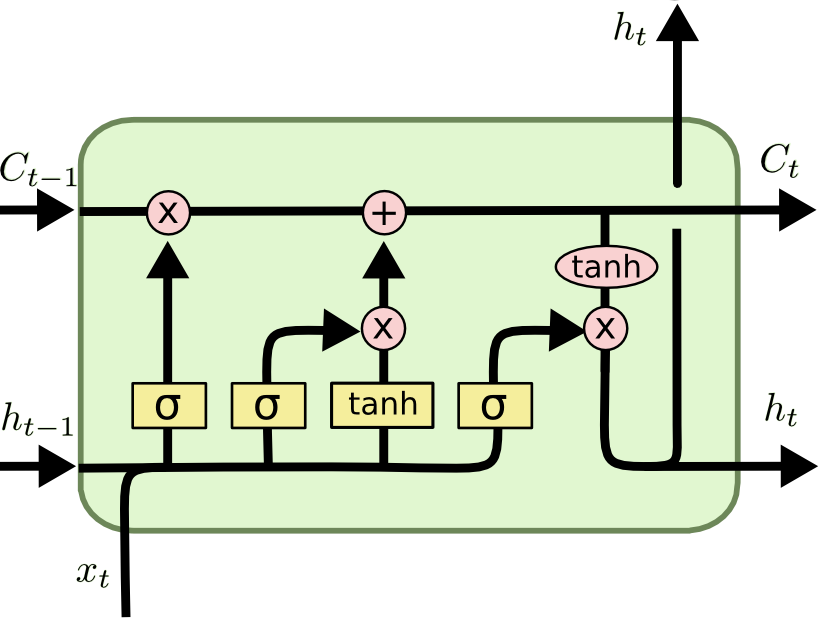
\includegraphics[width=.36\textwidth]{LSTM.png}\hfill
    \caption{LSTM cell scheme (Christopher Olah, 2015).}
    \label{fig:LSTM_cell}
\end{figure}

%-------------------------------------------------------------------------
\section{Methodology and Development}

%---------------------
\subsection{Dataset and Preprocessing}

Historical price data of Bitcoin are collected from Dukascopy Bank, an online Swiss bank that provides trading services including CFDs (contract for difference) for cryptocurrencies among many other financial services. The currency pair used is BTC/USD and the original format of the time series was OHLC-V (Open, High, Low, Close, Volume) ticks for the two-price and volume quotation: Bid, the highest price a buyer will pay, and Ask, the lowest price a seller will accept. However, for implementation reasons regarding the input of the LSTM, the average between each Ask and Bid price and also for Volume is computed, which gives a valid reference of the general price and volume in the spread.

Although Bitcoin officially started in 2009, the data available in this research was gathered from years 2017 to 2020 and contained more than 108 million ticks of transactions. Although it may seem like a lot of data, and definitely enough for the purpose of this study, it could mean a lack of data for more advanced and sophisticated systems due to the fact that samples have been reduced along the way in two steps: when grouping ticks by time bars and when generating sequences from samples to input the LSTM, as explained below.

It must be pointed out that the definition of the prediction horizon is key when constructing deep learning models. In fact, the majority of high-frequency trading systems use intraday price movements because, in general, the performance of daily short-range predictions is superior than weekly or monthly forecasts. For this purpose, 1-minute time bars are sampled from the ticks in the dataset in order to achieve the aforementioned granularity.

When performing this grouping of transaction ticks by time bars and getting the volume feature, the number of original samples shrank to little more than 1 million. Moreover, when generating the sequences from these samples to input the LSTM, the data reduced up to 124.391 sequences. Thus, it is important to be aware of the quantity of data to gather in order to meet the needs of your purpose. For this study, data from 2017-05 to 2020-01 is used for the training phase (about 78\% of data), the collection from 2020-01 to 2020-07 is used for validation (approximately 15\% of data) and the remaining set from 2020-07 up to 2020-10 is used for test data (about 7\% of data).

To the above, we add the observation that the financial markets present strong non-linearity and non-stationarity in their time series, meaning that moments will change over time. For that very reason, and in order to stabilize the mean and variance along the series, the relative log-return of the Close price (\ref{returns}) is used as the target variable to predict:

\begin{equation} \label{returns}
	r_i = \log(p_i) - \log(p_{i-10})
\end{equation}

In this way, returns can be assumed to be stationary and the prediction span of the model is set 10 minutes forward in time, for the same reasons mentioned above. The proposed model also uses another type of input: a set of 4 of the most common technical indicators used in the market and in related work. These added features pretend to provide a positive influence to the performance of the model in the sense that those kinds of patterns do not have to be learned by the network and overfitting is reduced. The technical indicators used are listed below:
\\\\
\indent\textbf{Bollinger Bands (BB)}.
Bollinger Bands are a volatility indicator composed of a middle band and an upper band that widens when standard deviation increases and a lower band that contracts when it decreases since volatility is essentially based on standard deviation. The middle band (\ref{BB}) is a simple moving average and is the only indicator that has been used for simplicity.

\begin{equation} \label{BB}
	\text{Middle Band} = \frac{1}{n} \sum_{i=0}^{n-1} p_{M-i}
\end{equation}

\textbf{Relative Strength Index (RSI)}.
The relative strength index (\ref{RSI}) is a momentum indicator, \ie a tool to determine the strength (overbought) or weakness (oversold) conditions of an asset’s price. It measures the speed and change of price (from 0 to 100) by comparing the magnitude of gains and losses over a specified period of time.

\begin{equation} \label{RSI}
	\text{RSI} = 100 - (\frac{100}{1+\frac{n_{\text{up}}}{n_\text{down}}})
\end{equation}

\textbf{Moving Average Convergence Divergence (MACD)}.
The moving average convergence-divergence (\ref{MACD}) is a momentum indicator based on exponential moving averages which compares the long and short average trends. The MACD oscillates above and below zero depending on whether the moving average converges or diverges. Note that even though it is useful to generate signals, it is not helpful for distinguishing overbought or oversold conditions because the indicator is unbounded.
\begin{align} \label{MACD}
	\text{MACD}_{k,l,m}^t &= \text{MME}_{k,\alpha}^t [\text{MME}_{l,\alpha}^t (T) - \text{MME}_{m,\alpha}^t (T)] \nonumber \\
	\text{MME}_k^t &= \lambda p_t + (1 - \lambda)\text{MME}_k^{t-1}
\end{align}

\textbf{Stochastic Oscillator (SO)}.
The stochastic oscillator (\ref{SO}) is an indicator of momentum sensitivity or price speed that measures the distance between the current price and the minimum-maximum range observed in $k$ sessions. The indicator is useful for distinguishing overbought or oversold conditions because of its boundness but, due to its instability and sometimes “false signals”, it is mainly used to detect market reversals.
\begin{equation} \label{SO}
	\text{SO}_k^t = \frac{p_t - \min_k^t}{\max_k^t - \min_k^t}
\end{equation}

Note the set of indicators described above are only used in almost half of the project experiments because, among other things, one of the objectives of the work is to compare the leverage of using or not technical indicators in such a model. On top of that, all input variables (OHLC-V prices and technical indicators), except for log-returns, are standardized to [-1,1] in order to avoid any scaling problem. This normalization step really helps the convergence of training and avoids numerical errors.

%---------------------
\subsection{Details of Implementation}

The way Recurrent Neural Networks process sequences, and therefore LSTMs, can be classified essentially as \textit{one-to-one}, \textit{many-to-one}, \textit{one-to-many} or \textit{many-to-many}. The first two approaches are also called single-step models, while the other two refer to multi-step models. As has already been mentioned in previous sections, the focus of this work is based on predicting the returns of the next 10 minutes given a previous fixed context of the temporal series; thus, it fits perfectly with a \textit{many-to-many} approach where the input is a sequence of $n$ values and the output is the prediction of $m$ consecutive values.

It must be clarified that the sequence length to feed the model depends on the nature of the data and its inner correlations, so there is no rule of thumb. Furthermore, back-propagation through time is not conducted to the whole series but usually to last steps, say 100-200. In fact, the sequence length does not really affect the training of the model but it compares as having more training examples in which just the previous state is kept instead of resetting it. And even with that, no notable improvements are shown when more context is fed into the network, since LSTMs mainly focus on last samples. Therefore, for the reasons stated above and in order to keep simplicity, sequences have been built by transforming samples into sequences of length 110, which context length is 100 and target length is 10 (corresponding to the 10 minute prediction given by the granularity of 1-minute bars).

Note that the sequence length has nothing to do with the input size, \ie the number of features used in the model. In this case, the input size does affect the complexity of the model, the number of parameters and hence the training time, so choosing which relevant features are used is important for the model's performance. Accordingly, the input size of the proposed model is 5 (\ie High, Low, Open, Close and Volume variables) as base for some trials and the input size is 9 (\ie OHLC-V plus technical indicators BB, RSI, MACD and SO) for other experiments in this work.

The architecture of the LSTM built with the PyTorch deep learning framework is formed by a single hidden layer and, therefore, it is composed of a recurrent layer (of dimensionality Input size $\times$ Hidden size) and a linear layer (of dimensionality Hidden size $\times$ Output size). The main point is that there is no rule for the number of hidden layers to use, as it is something that must be figured out for each case by trial and error. At the end, really deep networks at the cutting edge of research are really good to learn features at various levels of abstraction and at generalization, but shallow and wide neural networks are very good at memorization. Therefore, deep networks can be very computationally expensive to train.

There are two more main parameters that can be taken into account when defining the architecture of the LSTM such as the number of RNN layers and the bidirectional parameter. The former refers to the number of RNNs stacked on top of each other in order to get a multilayer network where a hidden from each layer and an output only from the topmost layer are given. The latter describes if the LSTM becomes a Bidirectional Long Short-Term Memory (BiLSTM) which runs the inputs two-way: one from the past to the future and another from the future to the past, hence using two hidden states combined and preserving information from both past and future. Due to the fact that stacked LSTMs greatly increase model’s complexity and the bidirectional approach does not seem appropriate for the financial series scenario, the number of layers is set to 1 and the bidirectionality to False. This way, the hyperparameters used to fine-tune the network are only batch size and hidden size.

\begin{table*}
\begin{center}
\begin{tabular}{ccccc|ccccc}
    \multicolumn{10}{c}{Validation data} \\
    \toprule
    Features & Step size (decay) & Hidden & Batch & Th. acc. & Features & Step size (decay) & Hidden & Batch & Th. acc. \\
    \midrule
    \cellcolor{lightgray}ohlcv + ti  & \cellcolor{lightgray}0.0001 (every 4 ep.) & \cellcolor{lightgray}32 & \cellcolor{lightgray}1024 & \cellcolor{lightgray}\textbf{54,20 \%} &  ohlcv + ti & 0.001 (every 8 ep.) & 128 & 256 & 49,31 \% \\
    \cellcolor{lightgray}ohlcv + ti & \cellcolor{lightgray}0.0001 (every 4 ep.) & \cellcolor{lightgray}32 & \cellcolor{lightgray}512 & \cellcolor{lightgray}\textbf{53,38 \%} & ohlcv & 0.0001 (every 4 ep.) & 128 & 256 & 49,27 \% \\
    \cellcolor{lightgray}ohlcv + ti & \cellcolor{lightgray}0.0001 (every 4 ep.) & \cellcolor{lightgray}32 & \cellcolor{lightgray}256 & \cellcolor{lightgray}\textbf{52,67 \%} & ohlcv + ti & 0.001 (every 8 ep.) & 64 & 512 & 49,25 \% \\
    ohlcv  & 0.0001 (every 4 ep.) & 64 & 512 & \textbf{52,23 \%} & ohlcv + ti & 0.001 (every 8 ep.) & 128 & 512 & 49,20 \% \\
    ohlcv & 0.001 (every 8 ep.) & 64 & 512 & \textbf{50,83 \%} & ohlcv & 0.001 (every 8 ep.) & 32 & 1024 & 48,83 \% \\
    ohlcv & 0.001 (every 8 ep.) & 32 & 512 & \textbf{50,65 \%} & ohlcv & 0.0001 (every 4 ep.) & 32 & 1024 & 48,77 \% \\
    ohlcv & 0.001 (every 8 ep.) & 128 & 256 & \textbf{50,44 \%} & ohlcv + ti & 0.001 (every 8 ep.) & 32 & 512 & 48,60 \% \\
    ohlcv & 0.001 (every 8 ep.) & 128 & 512 & \textbf{50,15 \%} & ohlcv + ti & 0.001 (every 8 ep.) & 32 & 256 & 48,41 \% \\
    ohlcv & 0.0001 (every 4 ep.) & 64 & 1024 & 49,85 \% & ohlcv + ti & 0.001 (every 8 ep.) & 64 & 1024 & 47,98 \% \\
    ohlcv & 0.001 (every 8 ep.) & 64 & 256 & 49,63 \% & ohlcv & 0.0001 (every 4 ep.) & 64 & 256 & 47,89 \% \\
    ohlcv & 0.001 (every 8 ep.) & 32 & 256 & 49,60 \% & ohlcv & 0.0001 (every 4 ep.) & 128 & 1024 & 47,71 \% \\
    ohlcv & 0.001 (every 8 ep.) & 128 & 1024 & 49,59 \% & ohlcv + ti & 0.001 (every 8 ep.) & 128 & 1024 & 47,69 \% \\
    ohlcv & 0.0001 (every 4 ep.) & 32 & 256 & 49,58 \% & ohlcv + ti & 0.0001 (every 4 ep.) & 64 & 512 & 47,67 \% \\
    ohlcv & 0.0001 (every 4 ep.) & 128 & 512 & 49,49 \% & ohlcv + ti & 0.001 (every 8 ep.) & 32 & 1024 & 47,50 \% \\
    ohlcv + ti & 0.001 (every 8 ep.) & 64 & 256 & 49,45 \% & ohlcv + ti & 0.0001 (every 4 ep.) & 64 & 256 & 46,44 \% \\
    ohlcv & 0.001 (every 8 ep.) & 64 & 1024 & 49,42 \% & ohlcv + ti & 0.0001 (every 4 ep.) & 128 & 256 & 45,33 \% \\
    ohlcv & 0.0001 (every 4 ep.) & 32 & 512 & 49,41 \% & ohlcv + ti & 0.0001 (every 4 ep.) & 128 & 512 & 44,84 \% \\
    ohlcv + ti & 0.0001 (every 4 ep.) & 64 & 1024 & 49,41 \% & ohlcv + ti & 0.0001 (every 4 ep.) & 128 & 1024 & 44,78 \% \\
    \bottomrule
    \end{tabular}
\end{center}
   \caption{Performance of models with different hyperparameter configurations, in validation data. "Th. acc." refers to the "threshold accuracy", \ie the accuracy considering only 1\% of predictions.}
   \label{all_models}
\end{table*}

Regarding the loss function used to evaluate the model, the most commonly used criterion in regression is applied, the Mean Square Error (MSE). The MSE measures the average or mean squared error of the predictions by calculating the square difference between the target and the prediction and averaging those values over the number of instances. In addition to this, it should be noted that in both training and validation phases, back-propagation through time (computing the derivative of the loss with respect the parameters or anything requiring gradients) is performed taking into account only the last $m$ samples of the output sequence, since it is the only part of the predicted sequence for which target labels are available. These last 10 samples correspond to the target length parameter set in the model.

The optimization algorithm used for training the model is the Adam algorithm which is an alternative to the traditional Stochastic Gradient Descent (SDG) method to iteratively update network weights more efficiently. The initial learning rate is set to the default value of 0.001 as base for some trials and 0.0001 for other experiments in this work. This step size is perhaps the most important hyperparameter to tune when configuring the network as it controls at what rate the model has to change in response to the predicted error every epoch, when weights are updated. Selecting a learning rate too large may create an unstable training and lead to learning suboptimal weights, while using a step size too small can make the training process take too long and get stuck in learning. In consequence, an adaptive learning rate approach is used when training by decaying its value by one order of magnitude every 4 or every 8 epochs, depending on the experiments performed. This strategy is implemented in order to prevent overfitting throughout the training phase.

%-------------------------------------------------------------------------
\section{Experiments}

To test the model, a series of experiments are conducted in order to fine-tune the network and determine the best hyperparameters that maximize the accuracy of predictions, \ie the correct price movements. First of all, for the purpose of building a baseline model, the least Mean Square Error is computed to compare with better models. The method is to obtain the optimal value that reduces the MSE in the worst case where the same value is predicted for all the samples; this optimal value is the average return of the target variable. Taking into account that returns are multiplied by a factor of 100, the baseline loss obtained based on MSE is 0.21 and 0.22 for the training and validation sets, respectively.

Besides that, and regarding model evaluation, it is needed not only to look at the generalization behaviour and potential of the model, which is provided by the scalar loss criterion, but also look at an evaluation metric that reflects the performance for the given goal. Even though the application of the study is not purely a classification problem but a kind of regression (because return values are predicted), it can be defined as a one in the sense that, simply by guessing which will be the movement of the price can be enough to obtain profits on trading, at least theoretically. So, the accuracy is used, which computes the fraction of correct sign predictions of returns.

However, this metric does not take into account the certainty of a given prediction, that is, how sure the forecast of a return is. It is clear that it is not the same to wrongly predict a big return when the actual return of the series was small than simply go over or below the true return just a little bit; the former has a huge impact on profitability. Therefore, in the financial field it is common to look only at the fraction of predictions that have the highest absolute value, \ie the ones that provide a higher return or profitability as well as higher certainty for a buy, hold or sell strategy on trading. The important thing is to get right when to buy and when to sell. This metric named here as “threshold accuracy” is computed by taking the accuracy of the 1\% of “safest” predictions. It will be clarified in the results when accuracy or “threshold accuracy” is being compared.

For the hyperparameter optimization, a series of exhaustive tests have been performed. In the first place, half of the experiments are performed using the four specified technical indicators and half of the tests without using them. Secondly, two approaches of learning rate behaviour are compared: one with an initial step size of 0.001 and a decay every 8 epochs, which can be defined to be “faster”, and a “slower” one with a starting step size of 0.0001 and a decay adjusted every 4 epochs. In third place, hidden size is tested on three values: 32, 64 and 128 (which seemed to work well on practice and related work), and batch size is originally tested on another three values: 256, 512 and 1024. However, when discarding parameter values that performed badly and choosing the final models, bigger batch sizes of 2048, 4096, 8192 and 16384 were also tested (further batch sizes could not be tested due to GPU memory issues).

All combinations of the above parameters are used to select the best model overall, in executions between 20 and 30 epochs of training.

On top of that, an additional strategy is used in order to deal with the induced randomness on model performance and robustness given by random seeds. Early experiments showed that random initialization of parameters such as weights and biases can adversely affect the consistency of models resulting in counterfactual interpretations. That is why 5 different seeds are used in all the experiments for which two things are done: 1- all final results metrics are averaged among the seeds and 2- a final ensemble model is built by averaging the output predictions of each model and each seed. This strategy is key and pertinent for the purpose of providing rigorous results.

%-------------------------------------------------------------------------
\section{Results}

When reviewing the results, it must be taken into account that, as a general rule in the financial context, outcomes above the 50\% threshold regarding the success of predictions are enough to consider a model suitable for its use. That is to say, guessing when to invest more and miss less implies a positive balance at the end of the period.

Table \ref{all_models} shows a summary of the performance of some models in the validation phase sorted by the value of “threshold accuracy”, \ie using only 1\% of predictions (the metrics are obtained by averaging all model executions among 5 different seeds and selecting the highest accuracy obtained in any of the epochs). It is important to note that only 8 of the tested models meet the requirements to become a suitable system, by being successful more than half the time. On the one hand, four main implications can be drawn from the table by paying attention to the top three models. The first one is that technical indicators generate a predictive lift up to 54\% in threshold accuracy in validation. The second is that using a “slower” learning rate initialized at 0.0001 and decayed every 4 epochs helps training. The third is that a small hidden size benefits the network. And the fourth one is that increasing batch size at every level improves the learning of the model.

On the other hand, it has to be said that obtaining these results has not occurred in the last epochs of training as would be expected in the learning curve. Instead, in many of the experiments the maximum accuracy was reached at the very first iterations. Moreover, the loss function presented the same behaviour and corroborated this effect. In comparison with the baseline training and validation loss (0.21 and 0.22 respectively), lower values were not barely reached when training in the sense that, if at one epoch the loss went down some decimals, it was still too close to the baseline. The above is not necessarily a problem for building a working model, but must be aware that this behaviour is closely related to overfitting. In any case, evidence of it will be given by the performance of the model in test data. 

\begin{table}[h]
\begin{center}
\begin{tabular}{ccc}
    \multicolumn{3}{c}{Validation data} \\
    \toprule
    Batch size & Accuracy & Threshold accuracy \\
    \toprule
    16384 & 50,17 \% & \cellcolor{lightgray}54,90 \% \\
    8192 & 50,16  \% & \cellcolor{lightgray}54,67 \% \\
    4096 & 50,15  \% & \cellcolor{lightgray}54,60 \% \\
    2048 & 50,08  \% & \cellcolor{lightgray}54,48 \% \\
    \bottomrule
    \end{tabular}
\end{center}
   \caption{Performance of four models in validation data using technical indicators, hidden size of 32 and a "slower" learning rate, and comparing the different batch sizes.}
\label{batch_models}
\end{table}

Given the best models obtained in the early tests of the study in the validation phase, the following parameters were fixed: using technical indicators, set the hidden size to 32, initializing the learning rate at 0.0001 and adjust it every 4 epochs (slow approach). Hence, increasing the batch size seemed to help the model performance. In fact, for a fixed number of training epochs, larger batches sizes take fewer steps, which translates into fewer parameter updates and shorter training times. There is no clear answer to when a higher batch size improves the model, but Table \ref{batch_models} shows the described effect (the metrics are obtained by averaging all model executions among 5 different seeds and selecting the highest accuracy obtained in any of the epochs). Increasing the batch size from 2048 up to 16384 slightly improves the model accuracy at every step.

The same conclusion is drawn when looking at the threshold accuracy, which naturally is always higher than accuracy. The important is that results show nearly a 55\% of threshold accuracy obtained in validation with the highest batch size.

\begin{table}[h]
\begin{center}
\begin{tabular}{cc}
    \multicolumn{2}{c}{Test data} \\
    \toprule
    Mean seed accuracy & 50,18 \% \\
    Mean ensemble accuracy & 50,47 \% \\
    \cellcolor{lightgray} Mean ensemble threshold accuracy & \cellcolor{lightgray}54,86 \% \\
    \bottomrule
    \end{tabular}
\end{center}
   \caption{Performance of the final ensamble model in test data using technical indicators, hidden size of 32 and a "slower" learning rate, and averaged over 5 seeds.}
\label{best_model}
\end{table}

%Example of a short caption, which should be centered.

Finally, Table \ref{best_model} shows the results obtained on test data using the model which obtained the highest accuracy, the one with batch size 16384. This final model is created by using an ensemble of 5 models with exactly the same parameters but different seeds. The “mean seed accuracy” refers to the average accuracy of each model separately and the “mean ensemble accuracy” refers to the accuracy of the ensemble which averages the predictions of each model. As it can be seen, the accuracy of 50.18\% confirms the value obtained in validation (50.17\%). In the end, the "mean ensemble threshold accuracy" of \textbf{54.86\%} is the most important one, as explained in previous sections. It can be defined as the ultimate metric to conclude the model performance. The presented results show that the architecture could make reasonable profit in trading strategies.

%-------------------------------------------------------------------------
\section{Conclusions and Future Work}

First and foremost, it is necessary to take into account the difficulty of predicting the daily profitability or return of a share given the almost zero autocorrelation of this data series. In fact, and regarding classical stock market analysis mechanisms, autoregressive models such as ARIMA and others do not work well against profitability in stock series. It is for that given reason that volatility models such as ARCH, GARCH and others are mainly used, which give estimates about risk (\ie volatility or standard deviation) but not forecasts about the direction of returns. However, in the application of this study, the problem to tackle is defined as the actual forecast of price returns of Bitcoin within the next 10 minutes, \ie obtaining 10 predictions of the value of returns 1 minute ahead in time, given that the granularity of the time series is given by 1-minute bars.

The proposed architecture of the LSTM (typically used in state-of-art language modeling deep learning tasks) can be considered very promising as it has proven to be able to predict well in comparison with other strategies employed and tested in the literature. Furthermore, results have shown that using a set of relevant technical indicators provide a positive influence to the performance of the model and it causes that these underlying trends and signals do not have to be learned by the network; thus, overfitting is reduced. In the same way, employing all the features available in the financial time series such as High, Low, Open, Close and Volume prices, which are the most relevant variables, enriches the model.

However, it is important to note that the experiments shown with an accuracy (or threshold accuracy) above 50\% do not necessarily guarantee that a profitable set of predictions is obtained for those models. On the one hand, the set of spreads, fees, commissions and other costs may cancel any profits, so it is vital to take them into account. On the other hand, because of the fact that the proposed models do not measure the volatility of the series nor use any kind of weighting to it, inducing mispredictions on major movements may lead to significant losses.

Finally, regarding the experience gathered in this study and focusing on future work, it must be highlighted the difficulty of withstanding the intrinsic complexity of dynamic and chaotic financial markets. This fact, combined with the low signal-to-noise ratio (SNR) that characterizes finance, makes the task of predicting stocks and cryptocurrencies market prices a very hard one. As Lopez de Prado describes in \cite{Prado}, some of the critical mistakes that must be taken into account when tackling quantitative finance problems with machine learning are: 1- avoid using time bars to process financial information, as key trading hours are more active than others in market sessions; 2- avoid learning side and size simultaneously, by referring “side” as the decision of whether to buy or sell and “size” as the risk management decision; and 3- avoid walk-forward (or historical) backtesting of only how a strategy would have performed in the past. These tips, combined with additional model architectures such as Convolutional Neural Networks (CNNs) or Reinforcement Learning (RL) strategies referred in related work provide a great opportunity for future research.

\newpage

{\small
\bibliographystyle{ieee_fullname}
\bibliography{egbib}
}

\end{document}
